\chapter{Introduction}
\paragraph{Summary} In this chapter, a short introduction to the topic of
computer vision is given. Thereafter, convolution is introduced. It is discussed
how (discrete) convolution can be written as a matrix product and the notion of
separability is discussed.

\section*{Overview}
Computer Vision is a very broad field with applications in many areas. For
instance, computer vision is
\begin{itemize}
\item useful in consumer devices (\eg fingerprint login on smartphone);
\item used as machine vision in quality control (\eg check that all pixels of a
  screen work which is a rather easy task, or to check that there are no
  scratches, which is a rather hard task);
\item making life-and-death decisions (\eg in autonomous emergency braking,
  cyclist and pedestrian detection. Applications in this area needs extremely
  high accuracy.
\end{itemize}
Considering the last point, an example procedure would be to take last $n$
frames (\eg $n = 11$) and decide based on them whether or not to brake. Clearly,
the false positive rate must be extremely low (\ie, do not want to brake if it
is not necessary). Additionally, we would like a low false negative
rate. Finally, the process should process the data in real-time which
corresponds to $\sim$ 30 megabyte of input per second.

Computer Vision is a compute-intensive endeavour and only two hand full of
algorithms are sufficiently efficient, \ie work at high scale and will make it
into consumer devices. We will therefore study these two hand full of algorithms
in-depth. They can then be combined in complicated pipelines. Although we will
study some of these pipelines we will mainly focus on the building blocks (see
Table~\ref{tab:ex:tasks}).

\begin{table}[htpb]
  \centering
  \begin{tabular}{lll}
    \toprule
    Input & Output & Task \\
    \midrule
    Image & 0/1 & Image classification \\
    Image & One class per pixel & Semantic/pixel segmentation \\
    Image & Which pixel belong to which instance & Instance segmentation \\
    Image & Pose of one or more humans & Pose estimation \\
    Video & Tracks of all targets & tracking \\ \bottomrule
  \end{tabular}
  \caption{Example tasks in computer vision}%
  \label{tab:ex:tasks}
\end{table}

\section[Convolution]{Linear Filters: Convolution}
Convolution is useful for
\begin{itemize}
\item Smoothing (Not SOTA)
\item Edge/Blob detection
\item General: Feature extraction
\end{itemize}
Has been mainstay of image analysis since it's very cheap (still matters now)
and is well-understood.

\subsection*{1D Convolution}
Consider the mean square estimator for $\{y_i\} \in \R$
\begin{gather*}
  \hat{y} = \argmin_y \sum_{i=1}^{n}{(y_i - y)}^2
\end{gather*}
that is given by (can be seen by letting the derivative of the sum above be
zero)
\begin{gather*}
  \hat{y} = \frac{1}{n} \sum_{i=1}^n y_i \,.
\end{gather*}
Using the same idea but introducing weights $w_i \ge 0$, \ie
\begin{gather*}
  \hat{y}_w = \argmin_y \sum_{i=1}^n w_i (y_i - y)^2
\end{gather*}
yields
\begin{gather*}
  \hat{y} = \frac{\sum_i w_i y_i}{\sum_i w_i}\,.
\end{gather*}
If, in addition, the weights depend on the distance from $x$ only, this can be
rewritten as (note that this no is a function of $x$)
\begin{gather*}
  \hat{y}_w(x) = \argmin_y \sum_{i=1}^n w_i(x - x_i) (y_i - y)^2
\end{gather*}
with solution
\begin{gather*}
  \hat{y}(x) = \frac{\sum_i w_i(x- x_i) y_i}{\sum_i w_i(x - x_i)}\,
\end{gather*}
and in the case of equidistant observations this simplifies to
\begin{gather*}
  \hat{y}_l = \frac{1}{\sum_i w_{l-i}}\sum_i w_{l-i} y_i\,,
\end{gather*}
which can be interpreted as the convolution of the signal $y$ and a weight
function $w$. The Figure below demonstrates the results of smoothing a perturbed
signal using two different weight functions, one being a NN kernel (that
corresponds to a characteristic function of an interval) and one being a
Epanechnikov kernel (that corresponds to a parabola that has been cut off at its
roots).

\begin{figure}[htpb]
  \centering 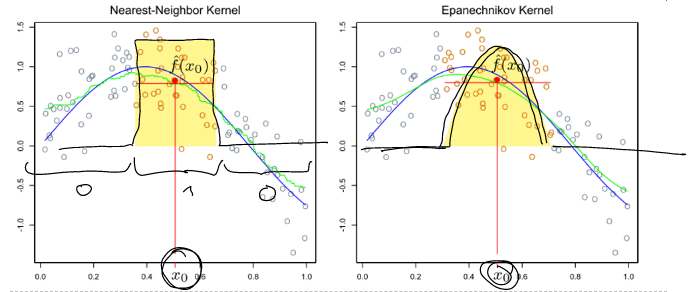
\includegraphics[width=0.9\textwidth,trim={0 1mm 0
    0},clip]{Figures/convolution_weight_examples.png}
  \caption{Box kernel and Epanechnikov kernel}%
  \label{fig:conv:kernel}
\end{figure}

Different filters can produce very different results ($\leadsto$ filter
optimisation). This is one instance of \emph{discrete convolution}
\begin{gather*}
  \sum_{i=0}^{n-1}f_{l-1}g_i \eqqcolon (f \ast g)_l
\end{gather*}
Properties:
\begin{itemize}
\item Convolution is \textbf{commutative}: $f \ast g = g \ast f$
\item Convolution is \textbf{associative}:
  $f \ast g \ast h = f \ast (g \ast h) = (f \ast g) \ast h$
  \begin{itemize}
  \item Important in practice, especially for image analysis
  \end{itemize}
\item Convolution is \textbf{distributive}:
  $f \ast (g + h) = f \ast g + f \ast h$
\end{itemize}
Important convolution filters include
\begin{itemize}
\item $f_i \ge 0$ smoothing (see above)
\item $f_i = \delta_{i-s}$ shifting
\item $f = 1/2(1 \ 0 \ -1)$ central finite difference (analogously non-central
  FD)
\item $f = [1\quad -1] \ast [1\quad -1] = [1\quad -2\quad 1]$ second derivative
\end{itemize}
Note: 1D convolution can be written as matrix multiplication with a
\emph{Töplitz matrix}
\begin{gather*}
  \sum_i f_{l-1}g_i \qquad \text{vs.} \qquad \sum_i M_{li}v_i = [M\cdot v]_r
\end{gather*}
Example: Consider the convolution
\begin{gather*}
  [1 \quad 0 \quad -1] \ast [g_0\quad g_1\quad g_2\quad g_3 \quad g_4] \\
  =
  \begin{bmatrix}
    0 & 1 & & & -1 \\
    -1 & 0 & 1 & & \\
    & -1 & 0 & 1 & \\
    & & -1 & 0 & 1 \\
    1 & & & -1 & 0
  \end{bmatrix}\cdot
  \begin{bmatrix}
    g_0 \\ g_1 \\ g_2 \\ g_3 \\ g_4\,,
  \end{bmatrix}
\end{gather*}
where the terms in the corners arise from periodic boundary conditions (\ie the
``$-1$-th'' term is the last term and the ``$n+1$-st'' term is the first term).

\subsection*{2D Convolution}
Convolution in higher dimensions can be defined analogously. Here, we have
\begin{gather*}
  \sum_i \sum_j f_{i,j}g_{u-i,v-j} \eqqcolon (f \ast g)(u,v)\,.
\end{gather*}
In image analysis $f$ is often small (\eg 3$\times$3) and $g$ large (\eg
3840$\times$2160).

Some filters are \textbf{separable} which means they can be written as an outer
product $f_{i,j} = a_i \cdot b_j$ This allows for storage reduction (instead of
storing the full matrix it suffices to store the vectors $a$ and
$b$)\footnote{Aside: Some filters are not separable but of low rank and using
  singular value decomposition we can find a suitable representation such as
  $f_{i,j} = \sum_{k=1}^r a_i^k b_j^k$ with $r$ small.}. In practice you would
use libraries because with the right memory layout, clever use of co-processors
and GPUs the speed can be drastically increased. If the filter is separable into
$a$ and $b$ as above, we can write
\begin{equation*}
  \underbrace{
    \sum_i a_i \underbrace{
      \sum_j b_j g_{u-i,v-j}
    }_{\text{1D convolution of rows}}
  }_{\text{1D convolution of columns}}
\end{equation*}

There are different options to extrapolate at the boundary of the image.


%%% Local Variables:
%%% mode: latex
%%% TeX-master: "../main"
%%% End:
